\section{Электронный транспорт в сверхрешётках (литературный обзор)}
\subsection{Квазиклассическое описание электронного транспорта в сверхрешётках}
Сверхрешётки представляют из себя твердотельные структуры, в которых помимо потенциала кристаллической решётки приложен внешний периодический потенциал, причём его период много больше периода кристаллической решётки. В зависимости от периодичности внешнего потенциала выделяют одно-, двух- и трёхмерные сверхрешётки.

Перейдём к описанию динамики электронов в одномерных сверхрешётках. Для определённости будем считать, что ось СР направлена вдоль оси \( z \). В приближении эффективной массы можно рассматривать электроны и дырки в полупроводнике как свободные частицы. Так же, как периодический потенциал кристаллической решётки приводит к разбиению непрерывного спектра свободных электронов на зоны, так и потенциал сверхрешётки разбивает разрешённые зоны на минизоны, разделённые минищелями, как показано на рисунке~\ref{fig:sl_spectrum}.
\begin{figure}[ht]
  \center
  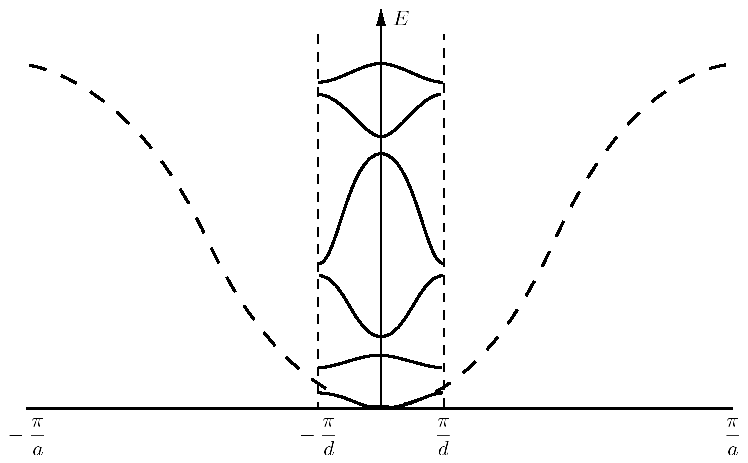
\includegraphics[width=.9\textwidth]{sl_spectrum}
  \caption{Минизонный спектр сверхрешётки. Периодический потенциал сверхрешётки приводит к разбиению зоны проводимости на минизоны, подобно тому, как потенциал решётки разбивает непрерывный спектр свободных электронов на зоны}
  \label{fig:sl_spectrum}
\end{figure}
Как правило, внешний потенциал имеет форму прямоугольных потенциальных ям, разделённых барьерами. Ширина минизон по порядку составляет \( 0,\!01 - 0,\!1~\text{эВ} \) и определяется вероятностью туннелировать из ямы в яму. В приближении сильной связи спектр электронов имеет вид
\begin{equation}
  \eps_{n}(\vec{p}) = \eps_{0n} + \frac{p_\perp^2}{2m^*} + \Delta_n \left( 1 - \cos\frac{p_z d}{\hbar} \right),
  \label{eq:sl_disp}
\end{equation}
где \( m^* \)~--- эффективная масса, \( \Delta_n \)~--- полуширина \( n \)-ой минизоны.

Поместим СР в электрическое поле, направленное параллельно оси. Суммарный потенциал уже не будет строго периодичен, поэтому применимость закона дисперсии \eqref{eq:sl_disp} зависит от соотношения между шириной минизоны и разностью энергии двух соседних периодов \( eEd \). Обычно физические явления, связанные с действием электрических полей на полупроводник не чувствительны к конечной ширине зоны проводимости, так как рассматриваемые поля обычно малы и рассеяние на неоднородностях решётки приводит к тому, что средняя энергия электронов мала по сравнению с шириной зоны. Однако, в СР ширина минизоны уже значительно меньше и средняя энергия электронов может оказаться больше её полуширины \( \Delta \). При нахождении электронов в верхней части минизоны уже начнёт существенно сказываться непараболичность спектра, которая приводит к тому, что СР начинают проявлять нелинейные оптические и электрические свойства в малых полях. Следствием непараболичности спектра является нелинейны отклик СР на воздействие внешних полей, например, нелинейная ВАХ и нелинейный радиоэлектрический эффект, а также существование в СР нелинейных периодических электромагнитных волн и солитонов. Нелинейность отклика также проявляется при совместном воздействии на СР сразу нескольких электромагнитных волн с различными (кратными) частотами. В этом случае не выполняется принцип суперпозиции: эффект их воздействия не сводится к сумме эффектов от каждой из волн в отдельности. Так, в сверхрешётках приложенное постоянное поле влияет на высокочастотную проводимость, а при падении двух волн наблюдаются эффекты двухволнового смешения и взаимного выпрямления. Многие из этих эффектов поддаются описанию в рамках квазиклассического подхода, в котором неравновесная функция распределения определяется из уравнения Больцмана, а потенциал СР приводит к ограничению пространства импульсов в соответствующем направлении. Этот подход оправдан в малых полях, когда \( eEd \ll \Delta \). В этом случае можно считать, что потенциал приложенного поля наклоняет минизону. Из-за этого электрон теперь может находиться лишь в области пространства протяжённостью \( 2\Delta / eE \), совершая в ней колебательное движение, что может быть объяснено в рамках предпринятого подхода.

Действительно, импульс электрона, находящегося в постоянном поле меняется со временем линейно:
\begin{equation*}
  p_z = p_{z0} + eEt.
\end{equation*}
Скорость электрона вдоль оси СР
\begin{equation*}
  v_z = \frac{d\Delta}{\hbar}\sin\frac{p_z d}{\hbar},
\end{equation*}
поэтому электрон совершает гармонические колебания с частотой \( \Omega = eEd/\hbar \). Качественно это можно объяснить следующим образом: двигаясь под действием электрического поля электрон перемещается в верхнюю часть минизоны, где эффективная масса становится отрицательной, и поле, раньше ускорявшее, начинает замедлять электрон. На границе зоны Бриллюэна электрон останавливается и возвращается в нижнюю часть минизоны. Такие колебания называются блоховскими осцилляциями, а частота \( \Omega \)~--- блоховской частотой. Макроскопический ток, получаемый усреднением по всему ансамблю, при этом равен нулю: \( j_z = 0 \). Но здесь не были учтены процессы рассеяния, которые обуславливают возникновение тока под действием внешних полей. В приближении постоянного времени релаксации ВАХ СР имеет вид
\begin{equation*}
  j_z = j_0\frac{\Omega\tau}{1+\Omega^2\tau^2}.
\end{equation*}
В малых полях, когда \( \Omega\tau \ll 1 \) или, что эквивалентно, \( E \ll \hbar / e\tau d \), \( j_z \sim E \) и для СР имеет место закон Ома. При \( \Omega\tau \gg 1 \) наблюдается отрицательная дифференциальная проводимость: \( j_z \sim 1/E \).

Приведённые выше выводы справедливы для любого кристалла с конечной шириной зоны проводимости. Однако, наблюдение блоховских осцилляций и отрицательной дифференциальной проводимости в обычных кристаллах практически невозможно. Условие \( \Omega\tau \gg 1 \) требует больших электрических полей, при которых с образцами происходили бы необратимые процессы. Для СР, период которых на 2 порядка больше периода кристаллической решётки, для наблюдения этих эффектов требуются значительно меньшие поля. С другой стороны, квазиклассический подход требует выполнения условия \( \hbar\Omega \ll \Delta \). Поэтому для наблюдения эффектов в СР должно выполняться условие
\begin{equation*}
  \Delta \gg \hbar / \tau,
\end{equation*}
из которого следует, что частота рассеяния носителей должна быть меньше штарковской.

Экспериментально блоховские осцилляции впервые были обнаружены в полупроводниковых СР квантовых ям на основе соединений \( \mathrm{Ga As / Al_x Ga_{1-x} As} \) \cite{feldmann}. Отрицательная дифференциальная проводимость в СР на основе \( \mathrm{GaAs/AlAs} \) экспериментально обнаружена и изучена в \cite{sibille}.

Исследования явлений отрицательной дифференциальной проводимости и блоховских осцилляций в СР вызваны широкими возможностями их применения на практике. Разработано множество экспериментальных методик на основе эффекта блоховских осцилляций и предложен ряд приборов \cite{andronov,elesin}. Отрицательная дифференциальная проводимость может быть использована для создания терагерцовых генераторов на основе таких структур. Возможность создания такого генератора рассматривается в работе \cite{andronov}. В \cite{suris} рассмотрены возможности применения СР в микроэлектронике в качестве фотодетекторов, каскадных и инжекционных лазеров). Также для генерации в терагерцовом диапазоне могут быть использованы блоховские осцилляции \cite{bouchard,martini}, что позволяет систематически экспериментально исследовать различные оптические нелинейные эффекты в этой частотной области \cite{keay}.

Одной из проблем, связанных с наблюдением блоховских осцилляций, является их затухание. В последнее время активно изучаются возможности подавления затухания. Так, в \cite{dmitriev} показана возможность значительного уменьшения затухания блоховских осцилляций в СР квантовых точек, а в \cite{suris-dmitriev} было получено квантовое кинетическое уравнение, которое описывает затухание блоховских осцилляций в идеальных СР квантовых точек. Затухание обуславливается процессами рассеяния, одним из главных механизмов которого является рассеяние на фононах. В работе \cite{suris-dmitriev} предложен способ существенно его уменьшить за счёт изменения электронного спектра под действием внешнего электрического поля.

Одно из первых исследований отрицательной дифференциальной проводимости в СР \cite{esaki} послужило поводом изучения этого явления в различных условиях. В \cite{mensah1} квазиклассическим методом исследовано влияние ионизации примесей электрическим полем на продольную ВАХ СР. Влияние высокочастотного поля на отрицательную дифференциальную проводимость изучено в \cite{ktitorov}. 

Как было показано ранее, воздействие постоянного поля на СР приводит к колебаниям носителей заряда. Но возможен и обратный эффект: появление постоянной составляющей тока под действием поля падающей волны \cite{alekseev}. Наблюдаемое выпрямление терагерцового поля является результатом процессов рассеяния и нелинейных процессов генерации самосогласованного поля под действием поля волны. Возникновение постоянной скорости у частиц является следствием спонтанного нарушения симметрии в такой системе. Оптическое выпрямление при совместном действии излучения большой мощности изучено в \cite{shmelev}.

Одновременное влияние на проводимость СР электромагнитного излучения и постоянного электрического поля интересно также в связи с тем, что действие электромагнитной волны может менять статическую ВАХ. При этом на ВАХ, как и в случае отсутствия электромагнитной волны, могут быть интервалы с отрицательной дифференциальной проводимостью. Кроме этого возможны области с абсолютной отрицательной проводимостью и состояния с нулевой проводимостью.

Нелинейные эффекты проявляются при одновременном действии постоянных и переменных полей. В \cite{unterrainer} теоретически и экспериментально исследовано совместное влияние влияние высокочастотного поля на блоховские осцилляции. В ВАХ полупроводниковой СР наблюдаются резонансные особенности, возникающие когда блоховская частота определенным образом соотносится с частотой излучения, приводящие к нулевой и абсолютной отрицательной проводимости. Также проводимость СР в условиях совместного действия переменного и постоянного электрических полей исследована в \cite{mensah2}, взаимодействие высокочастотных электрических полей в полупроводниковых СР изучена в \cite{bass}, а нелинейные оптические свойства СР~--- в \cite{ghosh}.

Эффекты нулевой и отрицательной проводимости, изученные в \cite{unterrainer} могут быть объяснены с точки зрения воздействия квантующего постоянного поля на спектр поглощения СР. Причиной нулевой проводимости и нулевого сопротивления в электронных системах также могут выступать постоянное магнитное поле и микроволновое излучение, совместно действующие на образец. Подробный обзор исследований абсолютной отрицательной проводимости таких электронных систем дан в \cite{red}.

Стоит также отметить, что в \cite{unterrainer}, где показана возможность существования абсолютной отрицательной проводимости и как следствие нулевой проводимости СР, вызванного совместным действием высокочастотного и постоянного электрических полей, пренебрегалось магнитным полем электромагнитной волны. Но в случае нулевой проводимости магнитное поля волны имеет решающее значение. Распространение волны вдоль СР вызывает эффект увлечения электронов, поэтому требует изучение совместное действие электромагнитной волны и постоянного поля в этом случае. Следовательно, необходимо рассмотрение конфигурации полей, при которой постоянное поле и направление распространения волны параллельны оси СР.

В \cite{pavlovich} исследован обратный эффект, заключающийся во влиянии внешнего электрического поля на высокочастотную проводимость полупроводников. При изучении нелинейной высокочастотной проводимость СР под действием постоянного электрического поля показано, что в области высоких частот под действием сильного постоянного электрического поля нелинейная высокочастотная проводимость меняет знак, т.е. поглощение волны сменяется усилением. В \cite{sivashova} показано, что в случае, когда вектор напряженности внешнего электрического поля перпендикулярен направлению распространения волны и параллелен напряженности электрического поля ЭМ излучения, эффектом увлечения так же можно управлять, изменяя внешнее постоянное электрическое поле. Причем смена знака радиоэлектрического эффекта сопровождается сменой знака высокочастотной проводимости СР.

Кроме совместного действия поля волны и постоянного электрического поля, интерес представляет взаимное действие нескольких электромагнитных волн на СР. В \cite{esaki} СР рассматривалась как новая искусственная нелинейная среда в которой возможны такие нелинейные оптические эффекты, как взаимное выпрямление и генерация гармоник. В \cite{bass} развита теория взаимодействия волн, основанная на решении уравнения Больцмана. Нелинейное взаимодействие ЭМ волн в СР приводит к возбуждение второй гармоники в случаях, когда первые гармоники распространяются в одну и в противоположные стороны \cite{bulgakov}. Там же проанализированы условия резонансного взаимодействия первой и второй гармоник. Изучение нелинейные высокочастотные явления в полупроводниковой СР привело к предсказанию ряда эффектов, таких как нелинейная зависимости тока увлечения от интенсивности волны, смена знака высокочастотной проводимости, взаимное усиление волн, самоиндуцированная прозрачность \cite{kechiev}.

Независимо в \cite{goychuk} изучена другая схема выпрямления. При совместном распространении электромагнитной волны и её второй гармоники условиями возникновения постоянного тока являются наличие квантового шума и пространственной периодичности системы.

В СР среди прочих нелинейных эффектов наблюдается эффект взаимного выпрямления, вызванный непараболичностью электронного спектра. Этот эффект описан в \cite{mensah} в квазиклассическом приближении с использованием кинетического уравнения Больцмана со столкновительным интегралом в приближении постоянного времени релаксации. Эффект состоит в появлении постоянного тока, возникающего в структурах с непараболичным законом дисперсии в результате наложения когерентных ЭМ волн с кратными частотами. Предполагалось, что частоты волн отличаются вдвое, волны распространяются поперек оси СР, а напряженность электрического поля осциллирует вдоль оси СР. Постоянная составляющая плотности тока вдоль этой оси СР нелинейно зависела от амплитуды гармоник.

Стоит отметить, что при определении тока двухволнового смешивания в \cite{mensah} рассматривались число синусоидальные волны, пренебрегая влиянием взаимодействия волны со СР на её форму. Проблема взаимного выпрямления волн в том случае, когда в СР присутствует не синусоидальное высокочастотное поле, как в \cite{mensah}, а волна, описываемая нелинейным уравнением, а именно уравнением синус-Гордона, рассмотрена в \cite{cnoidal-and-sinusoidal}.

В \cite{two-axis-sl} исследовано возникновение постоянного тока в полупроводниковой двухосевой СР под воздействием бихроматического электрического поля, поляризованного вдоль одной из осей, и влияние на него постоянного электрического поля, направленного вдоль другой оси. Зависимость постоянной составляющей плотности тока от напряженности постоянного поля носит резонансный характер: при приближении штарковской частоты к частоте одной из волн наблюдается резкое возрастание плотности тока, а при дальнейшем увеличении поля происходит резкая смена направления тока. Однако, двухосевая СР имеет периодический спектр как вдоль постоянного поля, так и вдоль высокочастотного, поэтому неясно, что именно обуславливает вид полученной зависимости.

\subsection{Графен и его свойства}
Графен был экспериментально обнаружен в 2004 г., но его свойства были исследованы теоретически задолго до открытия.

В двумерном графене атомы углерода периодически расположены в бесконечной гексагональной решетке. Такая атомарная структура определяется двумя типами связей при \( sp_2 \) гибридизации. Из 4 валентных орбиталей атома углерода (\(2s\), \(2p_x\), \(2p_y\) и \(2p_z\) орбитали, где направление \(z\) перпендикулярно листу), (\(s\), \(p_x\), \(p_y\)) орбитали объединяются, образуя в плоскости листа \(\sigma\) (связывающую или занятую) и \(\sigma^*\) (разрыхляющую или незанятую) орбитали. Эти орбитали плоские в соответствии с плоской симметрией. \(\sigma\)-связи являются сильными ковалентными связями, определяющими энергетическую устойчивость и упругие свойства графена. Оставшаяся \( p_z \) орбиталь, торчащая из плоскости листа, является непарной в соответствии с плоской симметрией и не связана с \(\sigma\)-состояниями. Из-за взаимодействия с соседними \( p_z \)-орбиталями (названного \(pp\pi\)-взаимодействием) формируются \(\pi\)- (связывающая) и \(\pi^*\)- (разрыхляющая) орбитали. Графит состоит из стопки многочисленных слоев графена. Примитивная ячейка в графите может быть прежде всего определена используя два слоя графена, сдвинутых друг относительно друга на расстояние между атомами углерода (\(a_{cc} = 1,\!42 \text{\AA}\)). Трехмерная структура графита поддерживается слабым межслоевым ван-дер-Ваальсовским взаимодействием между \(\pi\)-связями соседних слоев, которое вызывает слабую, но конечную делокализацию атомов из плоскости.

 Связывающие и разрыхляющие \(\sigma\)-зоны в действительности разделены большим энергетическим промежутком (> 12 эВ в \(\Gamma\)) и поэтому их вкладом в электронные свойства пренебрегают. Две оставшиеся \(\pi\)-зоны полностью описывают низкоэнергетическое электронное возбуждение как в графене, так и в графите. Связывающая \(\pi\) и разрыхляющая \(\pi^*\) орбитали образуют валентную зону и зону проводимости, пересекающиеся в точке электронейтральности (уровень Ферми в беспримесном графене) в вершинах гексагональной зоны Бриллюэна.

 Атомы углерода в слое графена расположены в вершинах гексагональной решетки. Эту решетку графена можно рассматривать как треугольную решетку Браве с двумя атомами в элементарной ячейке (A и B) и базисными векторами (\(\vec{a}_1, \vec{a}_2\)):
\[
    \vec{a}_1 = a\left\{\frac{\sqrt{3}}{2}, \frac{1}{2}\right\},
    \vec{a}_2 = a\left\{\frac{\sqrt{3}}{2}, -\frac{1}{2}\right\}.
\]
Обратите внимание, что \(a = \sqrt{3}a_{cc}\), где \(a_{cc} = 1,\!42 \text{\AA}\) -- расстояние между атомами углерода в графене. Каждый атом типа A или B окружен тремя атомами другого типа.

Векторы обратной решетки (\(\vec{b}_1, \vec{b}_2\)) могут быть получены, используя условие \(\vec{a}_i\cdot\vec{b}_j = 2\pi\delta_{ij}\),
\[
    \vec{b}_1 = b\left\{\frac{1}{2},\frac{\sqrt{3}}{2}\right\},
    \vec{b}_2 = b\left\{\frac{1}{2}, -\frac{\sqrt{3}}{2}\right\}.
\]
где \(b = 4\pi/(3a_{cc}) = 4\pi/a\sqrt{3}\). Шестиугольная зона Бриллюэна построена как ячейка Вигнера-Зейца в обратной решетке. Из шести ее углов только два не эквивалентны (остальные могут быть записаны в виде комбинации этих двух и векторов обратной решетки). Эти две точки отмечены \(K_+\) и \(K_-\). Другая симметричная точка отмечена буквой \( M \). Они могут быть выбраны следующим образом:
\[
    \vec{K}_+ = \frac{4\pi}{3a}\left\{\frac{\sqrt{3}}{2},-\frac{1}{2}\right\},
    \vec{K}_- = \frac{4\pi}{3a}\left\{\frac{\sqrt{3}}{2}, \frac{1}{2}\right\},
    \vec{M} = \frac{2\pi}{a\sqrt{3}}\left\{1,0\right\}.
\]
Элементарная ячейка и зона Бриллюэна графена приведены на рисунке~\ref{fig:graphene-lattices}.
\begin{figure}[ht]
  \center
  \includegraphics[width=.9\textwidth]{graphene-lattices}
  \caption{а) элементарная ячейка и б) зона Бриллюэна графена}
  \label{fig:graphene-lattices}
\end{figure}

Когда атомы углерода расположены в гексагональной решетке графена, волновые функции электронов от разных атомов перекрываются. Однако, в силу симметрии перекрытие между \(p_z\) орбиталями и \(s\) или \(p_x\) и \(p_y\) отсутствует. По этой причине \(p_z\)-электроны, формирующие \(\pi\)-связь в графене могут быть рассмотрены отдельно от других валентных электронов. В этом приближении атомы сорта A (или B) однозначно определяются одной орбиталью в каждом атоме \(p_z(\vec{r} — \vec{r}_A)\) (или \(p_z(\vec{r} — \vec{r}_B)\)).

Чтобы получить спектр гамильтониана, требуется решить соответствующее уравнение Шредингера. В соответствии с теоремой Блоха, собственные функции, вычисленные в двух данных узлах решетки Браве \(\vec{R}_i\) и \(\vec{R}_j\), отличаются друг от друга только на фазовый множитель \(\exp(i\vec{k}\cdot(\vec{R}_i — \vec{R}_j)\). Поскольку есть 2 типа атомов, то собственные функции представляют собой линейные комбинации блоховских сумм для каждой подрешетки:
\[
    \Psi(\vec{k},\vec{r}) =
    c_A(\vec{k})\tilde{p}_z^A(\vec{k}, \vec{r}) +
    c_B(\vec{k})\tilde{p}_z^B(\vec{k}, \vec{r}),
\]
где
\begin{gather*}
    \tilde{p}_z^A(\vec{k}, \vec{r}) = \frac{1}{\sqrt{N_{cells}}}
    \sum_j e^{i\vec{k}\cdot\vec{R}_j}
    p_z(\vec{r} - \vec{r}_A - \vec{R}_j),\\
    \tilde{p}_z^B(\vec{k}, \vec{r}) = \frac{1}{\sqrt{N_{cells}}}
    \sum_j e^{i\vec{k}\cdot\vec{R}_j}
    p_z(\vec{r} - \vec{r}_B - \vec{R}_j),\\
\end{gather*}
где \(\vec{k}\) -- волновой вектор электрона, \(N_{cells}\) -- число элементарных ячеек в листе графена, \(R_j\) -- узел решетки Браве.  Далее мы будем пренебрегать перекрытием \(s = \Braket{p_z^A|p_z^B}\) между соседними \(p_z\) орбиталями. Тогда блоховские суммы образуют ортонормированный базис:
\[
    \Braket{\tilde{p}_z^A(\vec{k})|\tilde{p}_z^B(\vec{k}')} = \delta_{\vec{k},\vec{k}'}\delta_{\alpha,\beta},
\]
где \(\alpha,\beta = A, B\). Используя эту ортогональность в уравнении Шредингера, \(\mathcal{H}\Psi(\vec{k},\vec{r}) = E\Psi(\vec{k},\vec{r}\), получим задачу на собственные значения:
\[
    \begin{pmatrix}
        \mathcal{H}_{AA}(\vec{k}) & \mathcal{H}_{AB}(\vec{k}) \\
        \mathcal{H}_{BA}(\vec{k}) & \mathcal{H}_{BB}(\vec{k})
    \end{pmatrix}
    \begin{pmatrix}
        c_A(\vec{k}) \\
        c_B(\vec{k})
    \end{pmatrix}
    =
    E(\vec{k})
    \begin{pmatrix}
        c_A(\vec{k}) \\
        c_B(\vec{k})
    \end{pmatrix}.
\]
Матричные элементы гамильтониана имеют вид:
\begin{gather*}
    \mathcal{H}_{AA}(\vec{k}) = \frac{1}{N_{cells}}
    \sum_{i,j} e^{i\vec{k}\cdot(\vec{R}_j-\vec{R}_i)}
    \Braket{p_z^{A,\vec{R}_i}|\mathcal{H}|p_z^{A,\vec{R}_j}},\\
    \mathcal{H}_{AB}(\vec{k}) = \frac{1}{N_{cells}}
    \sum_{i,j} e^{i\vec{k}\cdot(\vec{R}_j-\vec{R}_i)}
    \Braket{p_z^{A,\vec{R}_i}|\mathcal{H}|p_z^{B,\vec{R}_j}},
\end{gather*}
где \(\mathcal{H}_{AA}=\mathcal{H}_{BB}\) и \(\mathcal{H}_{AB}=\mathcal{H}_{BA}^*\), и введены обозначения \(p_z^{A,\vec{\tau}} = p_z(\vec{r} - \vec{r}_A — \vec{\tau})\) и \(p_z^{B,\vec{\tau}} = p_z(\vec{r} - \vec{r}_B — \vec{\tau})\). После простых преобразований, учитывая взаимодействие только с ближайшими соседями, получим:
\begin{align*}
    \mathcal{H}_{AB}(\vec{k}) & = \Braket{p_z^{A,0}|\mathcal{H}|p_z^{B,0}} + e^{-i\vec{k}\cdot\vec{a}_1}\Braket{p_z^{A,0}|\mathcal{H}|p_z^{B,-\vec{a}_1}} + e^{-i\vec{k}\cdot\vec{a}_2}\Braket{p_z^{A,0}|\mathcal{H}|p_z^{B,-\vec{a}_2}}\\
    & = -\gamma_0\alpha(\vec{k}),
\end{align*}
где \(\gamma_0\) учитывает интеграл переноса между ближайшими \(\pi\) орбиталями (типичные значения \(\gamma_0\) 2,9-3,1 эВ), а функция \(\alpha(\vec{k})\) имеет вид
\[
    \alpha(\vec{k}) = 1 + e^{-i\vec{k}\cdot\vec{a}_1} + e^{-i\vec{k}\cdot\vec{a}_2}.
\]

Принимая \( \Braket{p_z^{A,0}|\mathcal{H}|p_z^{A,0}} = \Braket{p_z^{B,0}|\mathcal{H}|p_z^{B,0}} = 0 \) за нулевой уровень энергии, мы можем записать \( \mathcal{H}(\vec{k}) \) так:
\begin{equation*}  
    \mathcal{H}(\vec{k}) = 
    \begin{pmatrix}
        0 & -\gamma_0\alpha(\vec{k})\\
        -\gamma_0\alpha(\vec{k})^* & 0
    \end{pmatrix}.
\end{equation*}
Этот гамильтониан очень привлекателен и может быть записан в обозначениях матриц Паули, подчеркивая аналогию со спиновым гамильтонианом. Дисперсионные соотношения для энергии просто получаемые из собственных значений \(\mathcal{H}(\vec{k})\), даются формулой:
\begin{align*}
    E_\pm(\vec{k}) & = \pm\gamma_0|\alpha(\vec{k})|\\
                   & = \pm\gamma_0\sqrt{3+2\cos(\vec{k}\cdot\vec{a_1})+2\cos(\vec{k}\cdot\vec{a_2})+2\cos(\vec{k}\cdot(\vec{a_2}-\vec{a_1}))},
\end{align*}
которая может быть расписана в виде
\begin{equation}
    E_\pm(k_x, k_y) = \pm\gamma_0\sqrt{1 + 4\cos\frac{\sqrt{3}k_xa}{2}\cos\frac{k_ya}{2} + 4\cos^2\frac{k_ya}{2}}.
    \label{eq:pi_disp}
\end{equation}
Зависимость энергии носителей от квазиимпульса, определяемая соотношением~\eqref{eq:pi_disp}, представлена на рисунке~\ref{fig:graphene-bands}.
\begin{figure}[ht]
  \center
  \includegraphics[width=.9\textwidth]{graphene-bands}
  \caption{Зонная структура графена. Валентная зона и зона проводимости соприкасаются в счётном множестве точек, поэтому графен принято называть полуметаллом}
  \label{fig:graphene-bands}
\end{figure}
Волновые векторы \(\vec{k} = (k_x, k_y)\) выбраны в первой шестиугольной зоне Бриллюэна. Очевидно, что нули \(\alpha(\vec{k})\) соответствует пересечению зон со знаками \(+\) и \(-\). Можно проверить, что \(\alpha(\vec{k} = \vec{K}_+) = \alpha(\vec{k} = \vec{K}_-) = 0\) и по этой причине пересечения происходят в точках \(\vec{K}_+\) и \(\vec{K}_-\). Более того, с одним \(p_z\) электроном на атом в \(\pi-\pi^*\) модели (три других \(s,p_x,p_y\) электрона заполняют лежащую ниже \(\sigma\) зону), зона (--) (зона с отрицательной энергией) полностью заполнена, в то время как (+) пустая, по крайней мере для электронейтрального графена. Таким образом, уровень ферми \( E_F \) (или точка электронейтральности) совпадает с нулем энергии и поверхность Ферми составлена из множества точек \(K_+\) и \(K_-\). Графен демонстрирует металлический (бесщелевой) характер. Однако,так как поверхность Ферми нульмерная (пока она сводится к дискретному и конечному набору точек), обычно используется понятие полуметалла или бесщелевого полупроводника. Рассмотрим \(\vec{k}\) в окрестности \(\vec{K}_+\) (или \(\vec{K}_-\)). В этих областях наблюдается линейная дисперсия для \(\pi\) и \(\pi^*\) зон:
\[
    E_\pm = \pm \hbar v_F |\delta\vec{k}|,
\]
где
\[
    v_F=\frac{\sqrt{3}\gamma_0 a}{2\hbar}
\]
групповая скорость электронов. Графен, таким образом, весьма специфичен из-за линейного соотношения между энергией и импульсом и электронно-дырочной симметрии. Электронные свойства вблизи углов зоны Бриллюэна похожи на свойства безмассовых дираковских фермионов формирующих ``дираковский конус''. Шесть точек, являющихся вершинами дираковских конусов называются дираковскими точками. Групповые скорости электронов вблизи этих точек достигают  \(~8,\!5\times10^5\) м/с и в аналогии с безмассовыми фермионами Дирака представляет эффективную ``скорость света''.

Такой характер дисперсионного соотношения позволяет описывать движение электронов вблизи дираковских точек уравнением Дирака. Действительно, гамильтониан вблизи точки \( K_+ \) имеет вид
\begin{equation}
      \mathcal{H}_+(\vec{k}) = 
      v_F
    \begin{pmatrix}
        0 & ik_x + k_y\\
        -ik_x + k_y & 0
    \end{pmatrix}.
    \label{eq:hamiltonian}
\end{equation}
Вблизи другой дираковской точки \( K_- \), гамильтониан принимает вид
\begin{equation*}
      \mathcal{H}_-(\vec{k}) = 
      v_F
    \begin{pmatrix}
        0 & ik_x - k_y\\
        -ik_x - k_y & 0
    \end{pmatrix}.
\end{equation*}

В низкоэнергетическом приближении состояния электронов вблизи различных дираковских точек можно считать независимыми. Поэтому гамильтониан должен быть составлен таким образом, чтобы \( \mathcal{H}_+ \) действовал только на состояния, локализованные около \( K_+ \), а \( \mathcal{H}_- \) действовал только на состояния, локализованные около \( K_- \). Поэтому гамильтониан имеет вид
\begin{equation*}
      \mathcal{H}(\vec{k}) = 
      \begin{pmatrix}
        \mathcal{H}_+ & 0\\
        0 & \mathcal{H}_-
    \end{pmatrix},
\end{equation*}
расписав который более подробно, получаем
\begin{equation*}
      \mathcal{H}(\vec{k}) = 
      v_F
      \left[
      \begin{pmatrix}
        -\sigma_2 & 0\\
        0 & -\sigma_2
    \end{pmatrix} k_x +
      \begin{pmatrix}
        \sigma_1 & 0\\
        0 & -\sigma_1
    \end{pmatrix} k_y
    \right],
\end{equation*}
где \( \sigma_1 \) и \( \sigma_2 \)~--- матрицы Паули:
\[
  \sigma_1 = \begin{pmatrix}
    0 & 1 \\
    1 & 0
  \end{pmatrix}, \quad
  \sigma_2 = \begin{pmatrix}
    0 & -i \\
    i & 0
  \end{pmatrix}.
\]

Рассмотрим теперь графен на подложке. Линейность спектра чистого бесконечного листа графена обеспечивается эквивалентностью двух его подрешёток. Если же лист поместить на подложку, то за счёт взаимодействия с ней симметрия может нарушиться и подрешётки перестанут быть эквивалентными. Это, в свою очередь, может привести к возникновению запрещённой зоны в графене. При этом электроны уже перестанут вести себя как безмассовые частицы, и приобретут некоторую массу. Графен, таким образом, станет полупроводником, причём ширина его запрещённой зоны будет зависеть от материала, из которого сделана подложка.

Получим выражение для спектра графена на подложке вблизи дираковских точек. В матрице \eqref{eq:hamiltonian} на диагонали стояли нули, что было обусловлено эквивалентностью подрешёток. Теперь из-за взаимодействия с подложкой, постоянная решётки которой отлична от постоянной решётки графена, потенциалы атомов углерода в различных подрешётках претерпевают различный сдвиг, который будем считать одинаковым для всех атомов в подрешётке. Поэтому гамильтониан \eqref{eq:hamiltonian} принимает вид
\begin{equation*}
      \mathcal{H}_+(\vec{k}) = 
      v_F
    \begin{pmatrix}
        U & ik_x + k_y\\
        -ik_x + k_y & V
    \end{pmatrix},
\end{equation*}
а его собственные значения
\begin{equation*}
  \eps = v_F\left[ \frac{U+V}{2} \pm \sqrt{\left(\frac{U-V}{2}\right)^2+k^2} \right].
\end{equation*}
Первое слагаемое в скобках может быть опущено, так как оно определяется уровнем отсчёта энергии. Обозначая \( v_F|U-V| = 2\Delta \), можем переписать спектр в виде
\begin{equation*}
  \eps = \pm\sqrt{\Delta^2 + v_F^2k^2}.
\end{equation*}
Положительные энергии соответствуют электронам проводимости, отрицательные -- дыркам. Между зоной проводимости и валентной зоной появляется щель шириной \( 2\Delta \), а спектр носителей уже соответствует спектру ``релятивистских'' частиц с массой \( \Delta / v_F^2 \) и ``скоростью света'' \( v_F \).

\subsection{Сверхрешётки на основе графена}
Сверхрешётки на основе графена могут быть созданы различными способами: как за счёт чередования слоёв графена со слоями подходящего диэлектрика (например, гексагонального нитрида бора), так и за счёт создания периодического внешнего потенциала, используя периодически размещённые контактные площадки \cite{olbrich}. Возможно создание ГСР при помощи периодического магнитного поля, а также при помощи размещения на его поверхности периодически расположенных атомов водорода. В чистом графене СР может быть образована за счёт ``рипплов''~--- волн, которыми изгибается графен в отсутствие подложки. Также возможно создание муаровых сверхрешёток, в которых периодический потенциал создаётся за счёт рассогласования решеток графена и подложки, либо за счёт поворота листов графена друг относительно друга на малый угол.

Но наиболее удобным в плане изготовления и применения, являются ГСР, периодический потенциал в которых создаётся за счёт взаимодействия с полосчатой подложкой \cite{ratnikov}. Засечёт различного взаимодействия графена со слоями подложки образуются потенциальные ямы, разделённые барьерами. В качестве одного из материалов можно взять \( \mathrm{SiO_2} \), взаимодействие с которым не приводит к образованию щели в графене, а в качестве второго~--- \( \mathrm{BN} \) или \( \mathrm{SiC} \), при взаимодействии с которыми в графене образуется запрещённая зона, 53 и 260 мэВ соответственно. Пример такой сверхрешётки приведён на рисунке~\ref{fig:sl-sio2-bn}.
\begin{figure}[ht]
  \center
  \includegraphics[width=0.9\textwidth]{sl-sio2-bn}
  \caption{Графеновая сверхрешётка на полосчатой подложке \( \mathrm{SiO_2/h-BN} \)}
  \label{fig:sl-sio2-bn}
\end{figure}

Спектр носителей в такой ГСР может быть рассчитан с использованием модели Кронига-Пенни. Дисперсионное соотношение имеет вид \cite{ratnikov}
\begin{equation*}
  \frac{v_F^2(k_2^2-k_1^2) + V_0^2 - \Delta^2}{2v_F^2k_1k_2}\sh(k_2d_2)\sin(k_1d_1) + \ch(k_2d_2)\cos(k_1d_1) = \cos(k_x d).
\end{equation*}
Численный анализ дисперсионного соотношения позволяет записать спектр в виде \cite{gsl-sio2-sic}
\begin{equation*}
  \eps_{appr} = \sqrt{\Delta_g^2 + v_F^2 p_y^2} + \frac{\Delta_g\Delta}{\sqrt{\Delta_g^2 + v_F^2 p_y^2}}\left(1-\cos\frac{p_x d}{\hbar}\right),
\end{equation*}
где \( \Delta_g \)~--- полуширина щели между нижней электронной и верхней дырочной минизонами, \( \Delta \)~--- полуширина минизоны.

Чтобы дополнительный периодический потенциал мог привести к разбиению зоны проводимости графена на минизоны, период сверхструктуры \(d\) должен быть много меньше, чем средняя длина свободного пробега в графене \(\lambda\): \(d \ll \lambda\), которая при комнатной температуре и концентрации носителей заряда \(n \sim 10^{12}~\text{см}^{-2}\) составляет \(\lambda \approx 4 \cdot 10^{-5}~\text{см} \) \cite{novoselov-geim}. Для достижения наибольшего отношения ширины запрещённой зоны к ширине разрешённой в сверхрешётке с использованием нитрида бора в качестве щелевой модификации период сверхструктуры \( d\approx0,\!2\lambda\), а при использовании в подложке карбида кремния период сверхрешетки должен составлять приблизительно \(d\approx0,\!05\lambda\). Поэтому ограничения одноминизонного приближения лучше выполняются в сверхрешетке на основе графена, помещенного на подложку, состоящую из чередующихся полосок оксида кремния и карбида кремния \cite{gsl-sio2-sic}.

\section{Влияние постоянного поля на взаимное выпрямление в графеновой сверхрешётке}
\subsection{Постановка задачи}
Для уточнения причин резонансной зависимости постоянного тока от поперечного постоянного поля в настоящей работе рассматривается влияние полей той же конфигурации на одноосевую СР на основе графена. Выбор графеновой СР обусловлен неаддитивностью спектра, которая также имеет место в рассмотренной в \cite{two-axis-sl} СР. Вопрос о причинах эффекта решается рассмотрением двух различных ориентаций поля относительно СР: в одном случае постоянное поле направлено поперек оси СР, а в другом~--- вдоль.

Рассмотрим падение двух монохроматичных линейно поляризованных волн на сверхрешётку, находящуюся в постоянном электрическом поле. Частота одной из волн вдвое больше частоты другой, плоскости поляризации совпадают, а постоянное поле перпендикулярно плоскости поляризации. При падении таких волн на сверхрешётку возникает постоянная составляющая тока вдоль поля \cite{mensah}, поэтому представляет интерес определить влияние поперечного постоянного поля на этот ток. Здесь возможны две ориентации полей относительно оси сверхрешётки, при которых задача несколько упрощается: либо высокочастотные поля направлены вдоль оси решётки, а постоянное поперёк, либо наоборот.

\subsection{Отклик на внешнее электрическое поле в приближении постоянного времени релаксации}
Расположим графеновую сверхрешётку в плоскости \( xOz \), направив ось
\( z \) вдоль оси сверхрешётки, как показано на рисунке~\ref{fig:sl}.
\begin{figure}[ht]
    \center
    \includegraphics[width=0.8\textwidth]{graphene}
    \caption{Геометрия задачи}
    \label{fig:sl}
\end{figure}
Спектр электронов можно приблизить выражением
\cite{gsl-sio2-sic}
  \begin{equation*}
    \eps(\vec{p}) = \sqrt{\eps_0^2 + v_F^2 p_x^2} +
    \frac{\eps_1^2}{\sqrt{\eps_0^2 + v_F^2 p_x^2}}\left(1-\cos\frac{p_z
    d}{\hbar}\right),
  \end{equation*}
  где \( \eps_0 = 0,\!059~\text{эВ} \), \( \eps_1 = 0,\!029~\text{эВ} \),
  \( d = 2 \cdot 10^{-6}~\text{см} \) -- период сверхрешётки, а
  \( v_F = 10^8~\frac{\text{см}}{\text{с}} \)\cite{cnoidal-and-sinusoidal}.
 Нас интересует постоянная составляющая плотности тока
  \begin{equation*}
    \langle j_x \rangle = \left\langle \int d^2 p  f(\vec{p}, t) \pder{\eps}{p_x} \right\rangle,\quad
    \langle j_z \rangle = \left\langle \int d^2 p  f(\vec{p}, t) \pder{\eps}{p_z} \right\rangle,
  \end{equation*}
  где скобки означают усреднение по времени. Функцию распределения рассмотрим в
  приближении постоянного времени релаксации \cite{kogan}:
  \begin{equation*}
    f(t) = \frac{1}{\tau}\int_{-\infty}^{t} dt' \exp\left(\frac{t'-t}{\tau}\right) f_0(\vec{p'}),
  \end{equation*}
  где
  \begin{equation*}
    f_0 = C\exp\left[-\frac{\eps(\vec{p})}{kT}\right]
  \end{equation*}
  есть равновесная функция распределения, а \( \vec{p'} \) удовлетворяет уравнению
  \begin{equation*}
    \der{\vec{p'}}{t'} = q\vec{E},\quad \vec{p'}(t) = \vec{p}.
  \end{equation*}
  Решение этого уравнения
  \begin{equation*}
  \begin{cases}
    p_x' = p_x + q\int_t^{t'}E_x(t_1) dt_1,\\ p_z' = p_z + q\int_t^{t'}E_z(t_1) dt_1.
  \end{cases}
  \end{equation*}
  Для удобства введём обозначения
  \begin{equation*}
    \xi = \frac{v_F}{\eps_0} p_x,\ \eta = \frac{p_z d}{\hbar},\ \alpha =
    \frac{t'-t}{\tau},\ \beta = \frac{\eps_0}{kT},
    \ \gamma = \frac{\eps_1^2}{\eps_0^2},
  \end{equation*}
  \begin{align*}
    & \kappa_x(\alpha, t) = \frac{v_F}{\eps_0}
      q\int_t^{t'}E_x(t_1) dt_1,\\
    & \kappa_z(\alpha, t) = \frac{d}{\hbar} q\int_t^{t'}E_z(t_1) dt_1.
  \end{align*}
  В этих обозначениях
  \begin{align*}
    \pder{\eps}{p_x}& = \frac{v_F^2 p_x}{\sqrt{\eps_0^2 + v_F^2 p_x^2}} -
      \frac{\eps_1^2v_F^2 p_x}{(\eps_0^2 + v_F^2
      p_x^2)^\frac{3}{2}}\left(1-\cos\frac{p_z d}{\hbar}\right) =
    \frac{v_F \xi}{\sqrt{1 + \xi^2}}\left( 1 - \frac{\gamma(1-\cos\eta)}{1 + \xi^2}\right),\\
    \pder{\eps}{p_z}& = \frac{d}{\hbar}\frac{\eps_1^2}{\sqrt{\eps_0^2 + v_F^2
    p_x^2}}\sin\frac{p_z d}{\hbar} =
    \frac{\gamma d}{\hbar}\frac{\eps_0}{\sqrt{1+\xi^2}}\sin\eta,
  \end{align*}
Подставляя в выражения для постоянных компонент тока, получаем
\begin{align*}
  \langle j_x \rangle =& \frac{C\eps_0\hbar}{d} \int_{-\infty}^\infty d\xi \int_{-\pi}^\pi d\eta \frac{\xi}{\sqrt{1 + \xi^2}}\left( 1 - \frac{\gamma(1-\cos\eta)}{1 + \xi^2}\right)
    \times\\\times&
\int_{-\infty}^{0} d \alpha e^\alpha\left\langle\exp\left[-\beta\sqrt{1+(\xi + \kappa_x)^2}\right]
  \exp\left[-\beta\gamma\frac{1-\cos(\eta + \kappa_z)}{\sqrt{1+(\xi + \kappa_x)^2}}\right]\right\rangle,\\
  \langle j_z \rangle =& \frac{C\gamma\eps_0^2}{v_F} \int_{-\infty}^\infty d\xi \int_{-\pi}^\pi d\eta \frac{\sin\eta}{\sqrt{1+\xi^2}}
    \times\\\times&
  \int_{-\infty}^{0} d \alpha e^\alpha\left\langle\exp\left[-\beta\sqrt{1+(\xi + \kappa_x)^2}\right]
  \exp\left[-\beta\gamma\frac{1-\cos(\eta + \kappa_z)}{\sqrt{1+(\xi + \kappa_x)^2}}\right]\right\rangle.
\end{align*}
Здесь от времени зависят только \( \kappa_1 \) и \( \kappa_2 \), поэтому усреднение производится только для выражений, в состав которых они входят. Так как интегрирование по \( \xi \) производится по бесконечным пределам, а по \( \eta \)~--- по периоду, то выполним замену переменных:
\begin{equation*}
  \xi \to \xi + \kappa_x,\quad \eta \to \eta + \kappa_z:
\end{equation*}
\begin{align*}
  \langle j_x \rangle =& \frac{C\eps_0\hbar}{d} \int_{-\infty}^\infty d\xi
  \exp\left[-\beta\left(\sqrt{1+\xi^2} + \frac{\gamma}{\sqrt{1+\xi^2}}\right)\right]
  \int_{-\pi}^\pi d\eta
  \exp\left[\frac{\beta\gamma\cos\eta}{\sqrt{1+\xi^2}}\right]
    \times\\\times&
  \int_{-\infty}^{0} d \alpha e^\alpha\left\langle\frac{\xi}{\sqrt{1 + (\xi-\kappa_x)^2}}\left( 1 - \frac{\gamma(1-\cos(\eta-\kappa_z))}{1 + (\xi-\kappa_x)^2}\right)\right\rangle,\\
  \langle j_z \rangle =& \frac{C\gamma\eps_0^2}{v_F} \int_{-\infty}^\infty d\xi \exp\left[-\beta\left(\sqrt{1+\xi^2} + \frac{\gamma}{\sqrt{1+\xi^2}}\right)\right]
  \int_{-\pi}^\pi d\eta \exp\left[\frac{\beta\gamma\cos\eta}{\sqrt{1+\xi^2}}\right]
    \times\\\times&
  \int_{-\infty}^{0}d \alpha e^\alpha\left\langle\frac{\sin(\eta-\kappa_z)}{\sqrt{1+(\xi-\kappa_x)^2}}\right\rangle.
\end{align*}
Теперь можно аналитически проинтегрировать по \(\eta\). Для этого потребуется взять 3 интеграла:
\begin{gather*}
  \int_{-\pi}^\pi d\eta e^{\mu\cos\eta} = 2\pi I_0(\mu),\quad
  \int_{-\pi}^\pi d\eta \sin(\eta - \kappa_z) e^{\mu\cos\eta} =
  -2\pi I_1(\mu)\sin\kappa_z,\\
  \int_{-\pi}^\pi d\eta \cos(\eta - \kappa_z) e^{\mu\cos\eta} =
  2\pi I_1(\mu)\cos\kappa_z,
\end{gather*}
где введено новое обозначение
\begin{equation*}
  \mu = \frac{\beta \gamma}{\sqrt{1+\xi^2}}.
\end{equation*}
В итоге получаем следующие выражения:
\begin{align*}
  \langle j_x \rangle =& 2\pi \frac{C\eps_0\hbar}{d} \int_{-\infty}^\infty d\xi \exp\left[-\beta\left(\sqrt{1+\xi^2} + \frac{\gamma}{\sqrt{1+\xi^2}}\right)\right]
    \times\\\times&
    \int_{-\infty}^{0} d \alpha e^\alpha\left\langle\frac{\xi}{\sqrt{1 + (\xi-\kappa_x)^2}}\left( I_0(\mu) - \frac{\gamma(I_0(\mu)-I_1(\mu)\cos\kappa_z)}{1 + (\xi-\kappa_x)^2}\right)\right\rangle,\\
  \langle j_z \rangle =& 2\pi \frac{C\gamma\eps_0^2}{v_F} \int_{-\infty}^\infty d\xi \exp\left[-\beta\left(\sqrt{1+\xi^2} + \frac{\gamma}{\sqrt{1+\xi^2}}\right)\right]
    \times\\\times&
    \int_{-\infty}^{0}d \alpha e^\alpha\left\langle\frac{-I_1(\mu)\sin\kappa_z}{\sqrt{1+(\xi-\kappa_x)^2}}\right\rangle.
\end{align*}
Без конкретного вида полей дальнейшее упрощение выражений невозможно. Перейдём к рассмотрению интересующих нас конфигураций полей.

\subsection{Влияние постоянного поля на продольное выпрямление}
Рассмотрим случай, когда плоскость поляризации параллельна оси СР, а постоянное поле прикладывается перпендикулярно. Этот случай изображён на рисунке~\ref{fig:geometry1}.
\begin{figure}[!h]
    \center
    \includegraphics[width=0.9\textwidth]{graphene1}
    \caption{Геометрия задачи}
    \label{fig:geometry1}
\end{figure}

Выпишем компоненты полей
\begin{equation*}
  E_x = E_0,\quad E_z = E_1\cos\omega t + E_2\cos2\omega t.
\end{equation*}
В этом случае
\begin{align*}
    &\kappa_x(\alpha, t) = \frac{v_F}{\eps_0}qE_0\alpha\tau,\\
    &\kappa_z(\alpha, t) = \frac{d}{\hbar} \frac{q}{2\omega}\left(2E_1(\sin\omega t' - \sin\omega t) + E_2(\sin2\omega t' - \sin2\omega t)\right),
\end{align*}
а интересовать нас будет ток вдоль оси z. Рассмотрим усредняемое выражение и учтём, что \(\kappa_x\) не зависит от \(t\):
\begin{equation*}
  \left\langle\frac{-I_1(\mu)\sin\kappa_z}{\sqrt{1+(\xi-\kappa_x)^2}}\right\rangle = \frac{-I_1(\mu)}{\sqrt{1+(\xi-\kappa_x)^2}}\langle\sin\kappa_z\rangle.
\end{equation*}
Немного преобразуем \( \kappa_z \):
\begin{equation*}
  \kappa_z = \frac{d}{\hbar} \frac{q}{\omega}\left[2E_1 \sin\frac{\alpha\omega\tau}{2}\cos\left(\omega t + \frac{\alpha\omega\tau}{2}\right) + E_2\sin\alpha\omega\tau\cos\left(2\omega t + \alpha\omega\tau\right)\right].
\end{equation*}
Введём обозначения
\begin{equation*}
  \delta = \frac{\alpha\omega\tau}{2},\quad
  \theta = \omega t + \delta,\quad
  e_1 = 2\frac{qE_1d}{\hbar\omega}\sin\delta,\quad
  e_2 = \frac{qE_2d}{\hbar\omega}\sin2\delta,\quad
  \omega_0 = \frac{v_F}{\eps_0}qE_0,
\end{equation*}
в которых выражение примет вид
\begin{equation*}
  \kappa_z = e_1\cos\theta + e_2\cos2\theta.
\end{equation*}
Теперь немного преобразуем усредняемое выражение:
\begin{equation*}
  \sin(e_1\cos\theta + e_2\cos2\theta) =
  \sin(e_1\cos\theta)\cos(e_2\cos2\theta) +
  \cos(e_1\cos\theta)\sin(e_2\cos2\theta),
\end{equation*}
\begin{equation*}
  \langle\sin\kappa_z\rangle =
  \langle\sin(e_1\cos\theta)\cos(e_2\cos2\theta)\rangle +
  \langle\cos(e_1\cos\theta)\sin(e_2\cos2\theta)\rangle.
\end{equation*}
Продолжим, раскладывая в ряды Фурье синусы и косинусы:
\begin{align*}
  &\cos(z\cos x) = J_0(z) + 2\sum_{n=1}^\infty (-1)^n J_{2n}(z)\cos2nx,\\
  &\sin(z\cos x) = 2\sum_{n=1}^\infty (-1)^{n+1} J_{2n-1}(z)\cos(2n-1)x.
\end{align*}
Заметим также, что
\begin{equation*}
    \langle \cos nx \cdot \cos mx \rangle = \frac{\delta_{mn}+\delta_{-mn}}{2}.
\end{equation*}
Подставляя ряды и усредняя, получаем
\begin{gather*}
  \langle\sin(e_1\cos\theta)\cos(e_2\cos2\theta)\rangle = \Bigg\langle2\sum_{m=1}^\infty (-1)^{m+1} J_{2m-1}(e_1)\cos(2m-1)\theta\times\\\times\left(J_0(e_2) + 2\sum_{n=1}^\infty (-1)^n J_{2n}(e_2)\cos4n\theta\right)\Bigg\rangle = 0,
\end{gather*}
\begin{gather*}
  \langle\cos(e_1\cos\theta)\sin(e_2\cos2\theta)\rangle =
  \Bigg\langle\left(J_0(e_1) + 2\sum_{n=1}^\infty (-1)^m
  J_{2m}(e_1)\cos2m\theta\right)\times\\\times2\sum_{n=1}^\infty (-1)^{n+1}
  J_{2n-1}(e_2)\cos2(2n-1)\theta\Bigg\rangle = 2\sum_{n=1}^\infty (-1)^n
  J_{4n-2}(e_1)J_{2n-1}(e_2).
\end{gather*}
Собирая всё вместе, получаем
\begin{gather*}
  \langle\sin\kappa_z\rangle =
  2\sum_{n=1}^\infty (-1)^n J_{4n-2}(e_1)J_{2n-1}(e_2)=\\=
  2\sum_{n=1}^\infty (-1)^n
  J_{4n-2}\left(2\frac{d}{\hbar}\frac{q}{\omega}E_1\sin\frac{\alpha\omega\tau}{2}\right)J_{2n-1}\left(\frac{d}{\hbar}\frac{q}{\omega}E_2\sin\alpha\omega\tau\right).
\end{gather*}
Аргументами функций Бесселя являются периодические функции, поэтому их можно разложить в ряды Фурье
\begin{align*}
    & J_{2n}(2z\sin\phi) =
    (-1)^n\sum_{m=-\infty}^\infty J_{m+n}(z)J_{m-n}(z) e^{i2m\phi},\\
    & J_{2n-1}(2z\sin\phi) =
    i(-1)^{n}\sum_{m=-\infty}^\infty J_{m-n}(z)J_{m+n-1}(z)e^{i(2m-1)\phi},
\end{align*}
откуда
\begin{gather*}
   \langle\sin\kappa_z\rangle =
  2\sum_{n=1}^\infty (-1)^n
  J_{4n-2}\left(2\frac{d}{\hbar}\frac{q}{\omega}E_1\sin\frac{\alpha\omega\tau}{2}\right)
  J_{2n-1}\left(\frac{d}{\hbar}\frac{q}{\omega}E_2\sin\alpha\omega\tau\right)
  =\\=
  -2i\sum_{n=1}^\infty\sum_{m=-\infty}^\infty\sum_{k=-\infty}^\infty
   J_{m+2n-1}(z_1)J_{m-2n+1}(z_1)J_{k-n}(z_2)J_{k+n-1}(z_2)e^{i(m+2k-1)\phi}=\\=
   -2i\sum_{m=-\infty}^\infty S_{m}(z_1,z_2) e^{im\phi} = 4\sum_{m=1}^\infty
   S_m(z_1,z_2)\sin m\phi,
\end{gather*}
где введены дополнительные обозначения
\begin{equation*}
    z_1 = \frac{qE_1d}{\hbar\omega},\quad
    z_2 = \frac{qE_2d}{2\hbar\omega},\quad
    \phi = \alpha\omega\tau,
\end{equation*}
\begin{equation*}
    S_m(z_1,z_2) = \sum_{n=1}^\infty\sum_{k=-\infty}^\infty
   J_{m-2k+2n}(z_1)J_{m-2k-2n+2}(z_1)J_{k-n}(z_2)J_{k+n-1}(z_2).
\end{equation*}
С усреднением закончили, теперь перейдём к интегралу по \(\alpha\):
\begin{equation*}
    \int_{-\infty}^{0}d \alpha
    e^\alpha\left\langle\frac{-I_1(\mu)\sin\kappa_z}{\sqrt{1+(\xi-\kappa_x)^2}}\right\rangle
    = 4I_1(\mu) \sum_{m=1}^\infty S_m(z_1,z_2) \int_0^\infty d \alpha
    \frac{e^{-\alpha}\sin m\alpha\omega\tau}{\sqrt{1+\left(\xi+\omega_0\tau\alpha\right)^2}}.
\end{equation*}
Введём для удобства функцию
\begin{equation*}
    R_m(a,b,c) = \int_0^\infty \frac{e^{-x}\sin
    (mcx)}{\sqrt{1+\left(a+bx\right)^2}}\,dx.
\end{equation*}
В итоге для постоянной составляющей продольного тока получается следующее выражение
\begin{align*}
    \langle j_z \rangle &= 8\pi \frac{C\gamma\eps_0^2}{v_F}\sum_{m=1}^\infty
    S_m\left(\frac{qE_1d}{\hbar\omega},\frac{qE_2d}{2\hbar\omega}\right)\times\\&\times
    \int_{-\infty}^\infty d\xi \exp\left[-\beta\left(\sqrt{1+\xi^2} +
    \frac{\gamma}{\sqrt{1+\xi^2}}\right)\right]
    I_1\left(\frac{\beta\gamma}{\sqrt{1+\xi^2}}\right) R_m(\xi, \omega_0\tau,
    \omega\tau).
\end{align*}
Дальнейшее упрощение этого выражения связано с введением дополнительных ограничений и рассмотрено в разделе~\ref{sec:pereval}. Тем не менее, это выражение может быть использовано для численного расчёта, результаты которого представлены на рисунке~\ref{fig:jz}.
\begin{figure}[h!]
    \center
    \includegraphics[width=.7\textwidth]{jz}
    \caption{Зависимость продольного тока от поперечного поля. При малых частотах наблюдается монотонное убывание величины тока с ростом напряженности постоянного поля; при больших частотах наблюдается возрастание величины тока в малых полях сменяющееся убыванием}
    \label{fig:jz}
\end{figure}
Как видно из графиков, при малых частотах постоянное поле приводит к уменьшению тока вдоль оси СР. Это связано с тем, что поле разогревает электроны, увеличивая их энергию. Но чем дальше от дна зоны находится электрон, тем меньшую скорость вдоль оси СР он имеет при том же продольном импульсе. Уменьшение скорости электронов приводит к уменьшению тока.

При больших частотах, когда между последовательными актами рассеяния успевает произойти полное колебание, на графике появляется рост тока в малых полях. Его можно объяснить следующим образом: чем больше частота, тем меньше амплитуда колебаний импульса, поэтому электроны колеблются вблизи дна минизоны, где скорости невелики. Малое постоянное электрическое поле, разогревая электроны, выводит их ближе к середине минизоны, где продольные составляющие скорости выше, что и обуславливает рост тока. Дальнейшее его убывание имеет те же причины, что и в случае малых частот.

\subsection{Влияние постоянного поля на поперечное выпрямление}
Теперь рассмотрим случай, когда плоскость поляризации падающих волн перпендикулярна оси СР, а постоянное поле направлено вдоль оси. Конфигурация полей приведена на рисунке~\ref{fig:geometry2}, а компоненты полей имеют вид
\begin{equation*}
  E_z = E_0,\quad E_x = E_1\cos\omega t + E_2\cos2\omega t.
\end{equation*}
\begin{figure}[!h]
    \center
    \includegraphics[width=0.9\textwidth]{graphene2}
    \caption{Геометрия задачи}
    \label{fig:geometry2}
\end{figure}
В этом случае
\begin{align*}
    &\kappa_x(\alpha, t) =
    \frac{v_F}{\eps_0}\frac{q}{2\omega}\left(2E_1(\sin\omega t' - \sin\omega t)
    + E_2(\sin2\omega t' - \sin2\omega t)\right),\\
    &\kappa_z(\alpha, t) = \frac{d}{\hbar}qE_0\alpha\tau.
\end{align*}
Интересующий нас ток направлен вдоль оси \(x\):
\begin{gather*}
  \langle j_x \rangle = 2\pi \frac{C\eps_0\hbar}{d} \int_{-\infty}^\infty d\xi
    \exp\left[-\beta\left(\sqrt{1+\xi^2}+\frac{\gamma}{\sqrt{1+\xi^2}}\right)\right]
    \times\\\times\int_{-\infty}^{0}
    d \alpha e^\alpha\left\langle\frac{\xi}{\sqrt{1 + (\xi-\kappa_x)^2}}\left(
    I_0(\mu) - \frac{\gamma(I_0(\mu)-I_1(\mu)\cos\kappa_z)}{1 +
(\xi-\kappa_x)^2}\right)\right\rangle.
\end{gather*}
Для его определения требуется усреднить по времени следующие выражения:
\begin{equation*}
    M_1 = \left\langle\left[1 +
    (\xi-\kappa_x)^2\right]^{-\frac{1}{2}}\right\rangle \text{ и }
    M_2 = \left\langle\left[1 +
    (\xi-\kappa_x)^2\right]^{-\frac{3}{2}}\right\rangle,
\end{equation*}
где введены уже знакомые обозначения
\begin{equation*}
    \kappa_x = e_1\cos\theta + e_2\cos2\theta,\ e_1 =
    2\frac{v_F}{\eps_0}\frac{q}{\omega}E_1 \sin\frac{\alpha\omega\tau}{2},
    \ e_2 = \frac{v_F}{\eps_0}\frac{q}{\omega}E_2 \sin\alpha\omega\tau.
\end{equation*}
На первый взгляд, непонятно как проинтегрировать это выражение. Поэтому ограничимся рассмотрением малых полей и разложим усредняемые выражения в ряд Маклорена по \( \kappa_x \):
\begin{align*}
    \left[1 + (\xi-\kappa_x)^2\right]^{-\frac{1}{2}} & \approx
    \frac{1}{\sqrt{1+\xi^2}} +
    \frac{\xi}{\left(1+\xi^2\right)^\frac{3}{2}}\kappa_x +
    \frac{2\xi^2-1}{2\left(1+\xi^2\right)^\frac{5}{2}}\kappa_x^2+
    \frac{\xi(2\xi^2-3)}{2\left(1+\xi^2\right)^\frac{7}{2}}\kappa_x^3,\\
    \left[1 + (\xi-\kappa_x)^2\right]^{-\frac{3}{2}} & \approx
    \frac{1}{\left(1+\xi^2\right)^\frac{3}{2}} +
    \frac{3\xi}{\left(1+\xi^2\right)^\frac{5}{2}}\kappa_x +
    \frac{3(4\xi^2-1)}{2\left(1+\xi^2\right)^\frac{7}{2}}\kappa_x^2+
    \frac{5\xi(4\xi^2-3)}{2\left(1+\xi^2\right)^\frac{9}{2}}\kappa_x^3,
\end{align*}
откуда с учётом
\begin{align*}
    & \langle\kappa_x^n\rangle = \langle(e_1\cos\theta+e_2\cos2\theta)^n\rangle=
    \sum_{m=0}^n e_1^m e_2^{n-m} \langle  \cos^m\theta
    \cos^{n-m}2\theta\rangle
\end{align*}
имеем
\begin{equation*}
    \langle \kappa_x^2 \rangle = \frac{e_1^2 + e_2^2}{2},\quad
    \langle \kappa_x^3 \rangle = \frac{e_1^2e_2}{4},
\end{equation*}
\begin{align}
    & M_1 \approx
    \frac{1}{\sqrt{1+\xi^2}} +
    \frac{2\xi^2-1}{4\left(1+\xi^2\right)^\frac{5}{2}}(e_1^2 + e_2^2) +
    \frac{3\xi(2\xi^2-3)}{8\left(1+\xi^2\right)^\frac{7}{2}}e_1^2e_2,\label{eq:M1} \\
    & M_2 \approx
    \frac{1}{\left(1+\xi^2\right)^\frac{3}{2}} +
    \frac{3(4\xi^2-1)}{4\left(1+\xi^2\right)^\frac{7}{2}}(e_1^2 + e_2^2)+
    \frac{15\xi(4\xi^2-3)}{8\left(1+\xi^2\right)^\frac{9}{2}}e_1^2e_2.\label{eq:M2}
\end{align}
Теперь заметим, что при интегрировании по \( \xi \) интеграл от нечётных функций равен нулю, поэтому
\begin{gather*}
    \langle j_x \rangle = 2\pi \frac{C\eps_0\hbar}{d} \int_{-\infty}^\infty d\xi
    \exp\left[-\beta\left(\sqrt{1+\xi^2}+
    \frac{\gamma}{\sqrt{1+\xi^2}}\right)\right] \times \\ \times \int_{-\infty}^{0}
    d \alpha e^\alpha \left( \frac{3\xi^2(2\xi^2-3)I_0(\mu)}
    {8\left(1 + \xi^2\right)^\frac{7}{2}} -
    \frac{15\gamma\xi^2(4\xi^2-3)(I_0(\mu)-I_1(\mu)\cos\kappa_z)}
    {8\left(1 + \xi^2\right)^\frac{9}{2}}\right)e_1^2e_2.
\end{gather*}
После интегрирования по переменной \( \xi \) получаем выражение для постоянной составляющей тока в виде:
\begin{equation*}
    \langle j_x \rangle = \int_{-\infty}^0 d\alpha e^\alpha (C_0 +
    C_1\cos\kappa_z)e_1^2e_2,
\end{equation*}
где \( C_1 \) и \( C_2 \) не зависят от \( \alpha \):
\begin{align*}
    C_0 = & 2\pi \frac{C\eps_0\hbar}{d} \int_{-\infty}^\infty d\xi
    \exp\left[-\beta\left(\sqrt{1+\xi^2}+
    \frac{\gamma}{\sqrt{1+\xi^2}}\right)\right]\times\\\times&
    \left( \frac{3\xi^2(2\xi^2-3)}
    {8\left(1 + \xi^2\right)^\frac{7}{2}} -
    \gamma\frac{15\xi^2(4\xi^2-3)}
    {8\left(1 + \xi^2\right)^\frac{9}{2}}\right)
    I_0\left(\frac{\eps_1^2}{\eps_0 kT\sqrt{1+\xi^2}}\right),\\
    C_1 = & 2\pi \frac{C\eps_0\hbar}{d} \int_{-\infty}^\infty d\xi
    \exp\left[-\beta\left(\sqrt{1+\xi^2}+
    \frac{\gamma}{\sqrt{1+\xi^2}}\right)\right]\times\\\times&
    \gamma\frac{15\xi^2(4\xi^2-3)}
    {8\left(1 + \xi^2\right)^\frac{9}{2}}
    I_1\left(\frac{\beta\gamma}{\sqrt{1+\xi^2}}\right).
\end{align*}

Введём обозначение \( \omega_0 = qE_0d/\hbar \) (штарковская частота), \( \kappa_z = \alpha\omega_0\tau\).
Тогда интегрирование по \( \alpha \) состоит во взятии двух интегралов:
\begin{gather*}
    \int_0^\infty d\alpha e^{-\alpha}
    \sin^2\frac{\alpha\omega\tau}{2}\sin\alpha\omega\tau
    =\frac{1}{2}\int_0^\infty d\alpha e^{-\alpha} \sin\alpha\omega\tau
    -\frac{1}{4}\int_0^\infty d\alpha e^{-\alpha} \sin2\alpha\omega\tau =\\=
    \frac{1}{2}\frac{\omega\tau}{1+\omega^2\tau^2} -
    \frac{1}{2}\frac{\omega\tau}{1+4\omega^2\tau^2}.
\end{gather*}
и
\begin{gather*}
    \int_0^\infty d\alpha e^{-\alpha}\sin^2\frac{\alpha\omega\tau}{2}
    \sin\alpha\omega\tau\cos\alpha\omega_0\tau=\\=
    \frac{1}{2}\int_0^\infty d\alpha e^{-\alpha} \sin\alpha\omega\tau
    \cos\alpha\omega_0\tau
    -\frac{1}{4}\int_0^\infty d\alpha e^{-\alpha} \sin2\alpha\omega\tau
    \cos\alpha\omega_0\tau = \\ =
    \frac{\omega\tau}{2}\frac{1+(\omega^2-\omega_0^2)\tau^2}
    {[1+(\omega+\omega_0)^2\tau^2][1+(\omega-\omega_0)^2\tau^2]}-\\-
    \frac{\omega\tau}{2}\frac{1+(4\omega^2-\omega_0^2)\tau^2}
    {[1+(2\omega+\omega_0)^2\tau^2][1+(2\omega-\omega_0)^2\tau^2]}.
\end{gather*}
В итоге получаем следующее выражение для постоянной составляющей плотности тока при поперечном выпрямлении:
\begin{gather*}
    \langle j_x \rangle = 2\omega\tau
    \frac{v_F^3}{\eps_0^3}\frac{q^3}{\omega^3}E_1^2 E_2
    \cdot\Bigg[
        C_0\left(
            \frac{1}{1+4\omega^2\tau^2} -
            \frac{1}{1+\omega^2\tau^2}
            \right) +\\+
        C_1\Bigg(
            \frac{1+(4\omega^2-\omega_0^2)\tau^2}
            {[1+(2\omega+\omega_0)^2\tau^2][1+(2\omega-\omega_0)^2\tau^2]}-\\-
            \frac{1+(\omega^2-\omega_0^2)\tau^2}
            {[1+(\omega+\omega_0)^2\tau^2][1+(\omega-\omega_0)^2\tau^2]}
            \Bigg)
    \Bigg].
\end{gather*}
Графики этой зависимости для различных частот падающих волн представлены на рисунке~\ref{fig:jx}.
\begin{figure}[ht]
\begin{center}
    \includegraphics[width=.7\textwidth]{jx.pdf}
    \caption{Зависимости постоянной составляющей тока от продольного поля при поперечном выпрямлении. При больших частотах зависимость приобретает резонансный характер, что связано с действием ВЧ поля на носители, совершающие блоховские осцилляции}
    \label{fig:jx}
\end{center}
\end{figure}
Как видно из графиков, при малых частотах, как и в случае, рассмотренном в предыдущем разделе, постоянное поле приводит к уменьшению тока взаимного выпрямления по той же причине. Но в случае больших частот мы наблюдаем принципиально иную картину, которая имела место в двухмерной полупроводниковой СР в работе \cite{two-axis-sl}: при приближении штарковской частоты к частоте одной из волн наблюдается резонансное возрастание величины тока и резкая смена знака. Причины такого поведения можно объяснить следующим образом: продольное постоянное электрическое поле вызывает блоховские осцилляции, причём из-за неаддитивности спектра они происходят как вдоль оси СР, так и поперёк. Падающие волны при частотах, больших, чем частота рассеяния также вызывают колебания. Из-за существенной нелинейности связи скорости поперечного движения электронов и компонент импульса при приближении частот блоховских осцилляций к частотам ВЧ полей происходит появление постоянной составляющей тока.


Получим приблизительные значения нулей этой функции при \( \omega\tau\gg1 \).
Заметим, что они располагаются вблизи точек \( \omega_0 = \omega \) и \(
\omega_0 = 2\omega \).

Для удобства введём обозначение \( \sigma = C_0/C_1 \). Представим корень в виде
\( \omega_1 = \omega + \Delta\omega \) и подставим его в уравнение \( \langle
j_x \rangle = 0\):
\begin{equation*}
    -\frac{3\sigma}{4\omega^2\tau^2} +
    \frac{1+3\omega^2\tau^2}{(1+9\omega^2\tau^2)(1+\omega^2\tau^2)}-
    \frac{1-2\omega\Delta\omega\tau^2}{(1+4\omega^2\tau^2 -
    4\omega\Delta\omega\tau^2)}=0,
\end{equation*}
\begin{equation*}
    \Delta\omega\tau=\frac{9\sigma-1}{6\omega\tau},
\end{equation*}
\begin{equation*}
    \omega_1=\omega\left(1+\frac{9\sigma-1}{6\omega^2\tau^2}\right).
\end{equation*}

Аналогично рассуждая, получим \( \omega_2 = 2\omega + \Delta\omega \):
\begin{equation*}
    -\frac{3\sigma}{4\omega^2\tau^2} +
    \frac{1-4\omega\Delta\omega\tau^2}{1+16\omega^2\tau^2 -
    8\omega\Delta\omega\tau^2}-
    \frac{1-3\omega^2\tau^2}{(1+9\omega^2\tau^2)(1+\omega^2\tau^2)}=0,
\end{equation*}
\begin{equation*}
    \Delta\omega\tau=\frac{19 - 36\sigma}{12\omega\tau},
\end{equation*}
\begin{equation*}
    \omega_2=\omega\left(2+\frac{19-36\sigma}{12\omega^2\tau^2}\right).
\end{equation*}

\subsection{Бесстолкновительное приближение}
Пусть до включения полей система находилась в равновесии и в момент времени 0
включили поля. Тогда функция распределения будет определяться выражением
\begin{equation*}
    f(\vec{p}, t) = f_0\left(\vec{p} - q\int_0^t \vec{E} dt'\right),
\end{equation*}
и интересующий нас ток будет определяться выражением
\begin{gather*}
  \langle j_x \rangle = 2\pi \frac{C\eps_0\hbar}{d} \int_{-\infty}^\infty d\xi
    \exp\left[-\beta\left(\sqrt{1+\xi^2}+\frac{\gamma}{\sqrt{1+\xi^2}}\right)\right]
    \times\\\times\left\langle\frac{\xi}{\sqrt{1 + (\xi-\kappa_x)^2}}\left(
    I_0(\mu) - \frac{\gamma(I_0(\mu)-I_1(\mu)\cos\kappa_z)}{1 +
(\xi-\kappa_x)^2}\right)\right\rangle,
\end{gather*}
где
\begin{align*}
    &\kappa_x(t) =
    -\frac{v_F}{\eps_0}\frac{q}{2\omega}\left(2E_1\sin\omega t
    + E_2\sin2\omega t\right),\\
    &\kappa_z(t) = -\frac{d}{\hbar}qE_0t.
\end{align*}
Заметим, что \( \kappa_x(t) \) -- нечётная периодическая функция с периодом \(
2\pi/\omega \). Это означает, что \( \langle \kappa_x^{2n-1} \rangle = 0 \).
Используем полученные ранее ряды \eqref{eq:M1} и \eqref{eq:M2}, а также учтём,
что \( \langle \kappa_x^{2n-1} \cos\omega_0t \rangle = 0 \) так же по соображениям чётности. Поэтому
\begin{equation*}
    \langle j_x \rangle = 0.
\end{equation*}

\subsection{Приближение низких температур}
При температурах \( T \ll \eps_0 / k \approx 700~\text{К} \) выполняется условие \( \beta \gg 1 \) и для взятия интеграла по \( \xi \) можно воспользоваться методом перевала.

Метод перевала позволяет оценить интегралы вида
\begin{equation*}
    F(\lambda) = \int_{-\infty}^{+\infty} \Phi(x) e^{-\lambda\phi(x)}\,dx
\end{equation*}
при больших \( \lambda \). Если функция \(\phi(x)\) имеет единственный минимум в точке \( x_0 \), то основная часть интеграла лежит в окрестности этой точки.
Разложим \( \phi(x) \) в ряд Тейлора вблизи минимума:
\begin{equation*}
    \phi(x) = \phi(x_0) + \frac{\phi''(x_0)(x-x_0)^2}{2} + o((x-x_0)^2),
\end{equation*}
Пользуясь этим разложением, оценим интеграл
\begin{equation*}
    F(\lambda) \approx \int_{-\infty}^{+\infty} \Phi(x)
    e^{-\lambda\left(\phi(x_0) + \frac{\phi''(x_0)}{2}(x-x_0)^2\right)} dx
\end{equation*}
Если \( \Phi(x_0) \ne 0 \), так как экспонента отлична от нуля в малой области, то
\begin{equation*}
    F(\lambda) \approx \Phi(x_0)e^{-\lambda\phi(x_0)} \int_{-\infty}^{+\infty}
    e^{-\lambda\frac{\phi''(x_0)}{2}(x-x_0)^2} dx
\end{equation*}
Интеграл справа -- это интеграл Эйлера-Пуассона, поэтому
\begin{equation*}
    F(\lambda) \approx \Phi(x_0)e^{-\lambda\phi(x_0)}
    \sqrt{\frac{2\pi}{\lambda\phi''(x_0)}}.
\end{equation*}
Если же \(\Phi(x_0) = 0 \), то разложим её в ряд Тейлора
\begin{equation*}
    \Phi(x) = \Phi'(x_0)(x-x_0) + \frac{\Phi''(x_0)(x-x_0)^2}{2}
    + o((x-x_0)^2),
\end{equation*}
\begin{align*}
    F(\lambda) &\approx \Phi'(x_0)e^{-\lambda\phi(x_0)}
    \int_{-\infty}^{+\infty}(x-x_0) e^{-\lambda\frac{\phi''(x_0)}{2}(x-x_0)^2} dx + \\
    &+\frac{\Phi''(x_0)}{2}e^{-\lambda\phi(x_0)}
    \int_{-\infty}^{+\infty}(x-x_0)^2 e^{-\lambda\frac{\phi''(x_0)}{2}(x-x_0)^2} dx.
\end{align*}
Заметим, что
\begin{equation*}
    \int_{-\infty}^{+\infty} e^{-\alpha x^2} dx = \sqrt{\frac{\pi}{\alpha}},\quad
    \int_{-\infty}^{+\infty} xe^{-\alpha x^2} dx = 0,\quad
    \int_{-\infty}^{+\infty} x^2e^{-\alpha x^2} dx =\frac{1}{2} \sqrt{\frac{\pi}{\alpha^3}},\quad
\end{equation*}
\begin{equation*}
    F(\lambda) \approx\frac{\Phi''(x_0)}{4}e^{-\lambda\phi(x_0)}
    \sqrt{\frac{2^3\pi}{\lambda^3[\phi''(x_0)]^3}}=
    \Phi''(x_0)e^{-\lambda\phi(x_0)}
    \sqrt{\frac{\pi}{2\lambda^3[\phi''(x_0)]^3}}.
\end{equation*}


Исследуем функцию в показателе экспоненты:
\begin{equation*}
    \phi(\xi) = \sqrt{1+\xi^2} + \frac{\gamma}{\sqrt{1+\xi^2}},
\end{equation*}
график которой приведён на рисунке~\ref{fig:phi}.
\begin{figure}[ht]
    \center
    \includegraphics[width=.7\textwidth]{phi}
    \caption{Вид функции в показателе экспоненты}
    \label{fig:phi}
\end{figure}
Вблизи нуля она раскладывается в ряд Маклорена
\begin{equation*}
    \phi(\xi) = \phi(0) + \frac{\phi''(0)\xi^2}{2} + o(\xi^3) = 1+\gamma
    +\frac{(1-\gamma)\xi^2}{2} + o(\xi^3),
\end{equation*}
Используя это, оценим интеграл
\begin{align*}
    & \int_{-\infty}^\infty d\xi \exp\left[-\beta\left(\sqrt{1+\xi^2} +
    \frac{\gamma}{\sqrt{1+\xi^2}}\right)\right]
    \frac{\xi}{\sqrt{1 + (\xi-\kappa_x)^2}}\times\\\times&\left( I_0(\mu) -
    \frac{\gamma(I_0(\mu)-I_1(\mu)\cos\kappa_z)}{1 + (\xi-\kappa_x)^2}\right)=
    \Phi''(0)e^{-\beta(1+\gamma)}\sqrt{\frac{\pi}{2\beta^3(1-\gamma)^3}},
\end{align*}
где под функцией \( \Phi(\xi) \) имеется ввиду
\begin{equation*}
    \Phi(\xi) = \frac{\xi}{\sqrt{1 + (\xi-\kappa_x)^2}}\left( I_0(\mu) -
    \frac{\gamma(I_0(\mu)-I_1(\mu)\cos\kappa_z)}{1 + (\xi-\kappa_x)^2}\right),
\end{equation*}
\begin{align*}
    &\Phi'(\xi) = \frac{1}{\sqrt{1 + (\xi-\kappa_x)^2}}\left( I_0(\mu) -
    \frac{\gamma(I_0(\mu)-I_1(\mu)\cos\kappa_z)}{1 +(\xi-\kappa_x)^2}\right)-
    \\&-\xi(\xi-\kappa_x)\left(\frac{I_0(\mu)}{(1+(\xi-\kappa_x)^2)^\frac{3}{2}}-3
    \frac{\gamma(I_0(\mu)-I_1(\mu)\cos\kappa_z)}{(1 +
(\xi-\kappa_x)^2)^\frac{5}{2}}\right)-\\&-\frac{\beta\gamma\xi^2}{(1+\xi^2)^\frac{3}{2}\sqrt{1 + (\xi-\kappa_x)^2}}
\left( I_0'(\mu) - \frac{\gamma(I_0'(\mu)-I_1'(\mu)\cos\kappa_z)}{1
+(\xi-\kappa_x)^2}\right),
\end{align*}
\begin{align*}
    &\Phi''(0) = \kappa_x\left(\frac{I_0(\beta\gamma)}{(1+\kappa_x^2)^\frac{3}{2}}-3
    \frac{\gamma(I_0(\beta\gamma)-I_1(\beta\gamma)\cos\kappa_z)}{(1 + \kappa_x^2)^\frac{5}{2}}\right)+
    \\&+\kappa_x\left(\frac{I_0(\beta\gamma)}{(1+\kappa_x^2)^\frac{3}{2}}-3
    \frac{\gamma(I_0(\beta\gamma)-I_1(\beta\gamma)\cos\kappa_z)}{(1
    +\kappa_x^2)^\frac{5}{2}}\right)=\\
    &=2\kappa_x\left(\frac{I_0(\beta\gamma)}{(1+\kappa_x^2)^\frac{3}{2}}-3
    \frac{\gamma(I_0(\beta\gamma)-I_1(\beta\gamma)\cos\kappa_z)}{(1 +
    \kappa_x^2)^\frac{5}{2}}\right).
\end{align*}
В итоге, для поперечного тока получаем
\begin{align*}
    \langle j_x \rangle &=
    \frac{C\eps_0\hbar}{e^{\beta(1+\gamma)}d}\left[\frac{2\pi}{\beta(1-\gamma)}\right]^\frac{3}{2}\times \\
  &\times\int_{-\infty}^{0} d \alpha e^{\alpha} \left\langle
    \kappa_x\left[\frac{I_0(\beta\gamma)}{(1+\kappa_x^2)^\frac{3}{2}}-3\gamma
    \frac{I_0(\beta\gamma)-I_1(\beta\gamma)\cos\kappa_z}{(1 +
    \kappa_x^2)^\frac{5}{2}}\right]\right\rangle.
\end{align*}
А для продольного
\begin{align*}
  \langle j_z \rangle &= 2\pi \frac{C\gamma\eps_0^2}{v_F} \int_{-\infty}^\infty d\xi \exp\left[-\beta\left(\sqrt{1+\xi^2} + \frac{\gamma}{\sqrt{1+\xi^2}}\right)\right]\times\\&\times
    \int_{-\infty}^{0}d \alpha e^\alpha\left\langle
    \frac{-I_1(\mu)\sin\kappa_z}{\sqrt{1+(\xi-\kappa_x)^2}}\right\rangle \approx
    \\ &\approx
    2\pi\sqrt{\frac{\pi}{\beta(1-\gamma)}} \frac{C\gamma\eps_0^2}{v_F}
    I_1(\beta\gamma)e^{-\beta(1-\gamma)}
    \int_{-\infty}^{0}d \alpha e^\alpha\left\langle
    \frac{-\sin\kappa_z}{\sqrt{1+\kappa_x^2}}\right\rangle.
\end{align*}

\subsubsection{Случай продольного выпрямления}
\label{sec:pereval}
Снова выпишем для этого случая \( \kappa_x \)   и \( \kappa_z \):
\begin{align*}
    & \kappa_x(\alpha, t) = \alpha\omega_0\tau,\\
    & \kappa_z = e_1\cos\theta + e_2\cos2\theta,
\end{align*}
\begin{equation*}
  \delta = \frac{\alpha\omega\tau}{2},\quad
  \theta = \omega t + \delta,\quad
  e_1 = 2\frac{qE_1d}{\hbar\omega}\sin\delta,\quad
  e_2 = \frac{qE_2d}{\hbar\omega}\sin2\delta,\quad
  \omega_0 = \frac{v_F}{\eps_0}qE_0,
\end{equation*}
\begin{equation*}
    \langle j_z \rangle =
    2\pi\sqrt{\frac{\pi}{\beta(1-\gamma)}} \frac{C\gamma\eps_0^2}{v_F}
    I_1(\beta\gamma)e^{-\beta(1-\gamma)}
    \int_{-\infty}^{0}d \alpha e^\alpha
    \frac{-\langle\sin(e_1\cos\theta + e_2\cos2\theta)\rangle}{\sqrt{1+\alpha^2\omega_0^2\tau^2}}.
\end{equation*}
Отношение плотности тока в присутствии постоянного поля к плотности в отсутствие поля определяется выражением:
\begin{equation*}
    \frac{\langle j_z \rangle}{\langle j_{z0}\rangle}=\frac
    {\int\limits_0^{+\infty}d \alpha e^{-\alpha}
    \frac{\langle\sin(e_1\cos\theta +
    e_2\cos2\theta)\rangle}{\sqrt{1+\alpha^2\omega_0^2\tau^2}}}
    {\int\limits_0^{+\infty}d \alpha e^{-\alpha}
    \langle\sin(e_1\cos\theta + e_2\cos2\theta)\rangle}.
\end{equation*}
Результаты численного интегрирования представлены на графике ниже. Характер кривых тот же, что и при расчёте без использования метода перевала, однако, значения меньше на 10\%.
\begin{figure}[ht]
    \center
    \includegraphics[width=.7\textwidth]{jz_approx}
    \caption{Зависимость тока продольного взаимного выпрямления от поперечного постоянного поля}
\end{figure}

\subsubsection{Случай поперечного выпрямления}
В этом случае
\begin{align*}
    & \kappa_x = e_1\cos\theta + e_2\cos2\theta,\\
    &\kappa_z(\alpha, t) = \frac{d}{\hbar}qE_0\alpha\tau = \alpha\omega_0\tau,
\end{align*}
\begin{equation*}
    e_1 = 2\frac{v_F}{\eps_0}\frac{q}{\omega}E_1 \sin\frac{\alpha\omega\tau}{2},
    \ e_2 = \frac{v_F}{\eps_0}\frac{q}{\omega}E_2 \sin\alpha\omega\tau.
\end{equation*}
\begin{align*}
    \langle j_x \rangle &=
    \frac{C\eps_0\hbar}{e^{\beta(1+\gamma)}d}\left[\frac{2\pi}{\beta(1-\gamma)}\right]^\frac{3}{2}\times\\&\times
  \int_{-\infty}^{0} d \alpha e^{\alpha} \left\langle
    \kappa_x\left[\frac{I_0(\beta\gamma)}{(1+\kappa_x^2)^\frac{3}{2}}-3\gamma
    \frac{I_0(\beta\gamma)-I_1(\beta\gamma)\cos\alpha\omega_0\tau}{(1 +
    \kappa_x^2)^\frac{5}{2}}\right]\right\rangle.
\end{align*}
Характер кривых напоминает полученные ранее. Но нельзя не заметить, что теперь ток с ростом поля после скачков меняет направление на противоположное, в то время как ранее он был сонаправлен току в отсутствие постоянного поля. Значения в пиках превышают полученные ранее два раза.
\begin{figure}[ht]
    \center
    \includegraphics[width=.7\textwidth]{jx_approx}
    \caption{Зависимость тока поперечного взаимного выпрямления от продольного постоянного поля}
\end{figure}

\subsection{Условия экспериментального наблюдения эффекта}
Обсудим условия экспериментального наблюдения эффекта. Одноминизонное приближение накладывает определенные ограничения на частоту падающих волн, величину полей и температуру:
\begin{equation}
  \hbar\omega \ll \Delta_1,\quad eEd \ll \hbar\omega,\quad kT \ll \Delta_g
\end{equation}
где \( \Delta_1 \)~--- зазор между электронными минизонами, \( \Delta_g \)~--- ширина запрещённой зоны между нижней электронной и верхней дырочной минизонами. В рассматриваемой ГСР \( \Delta_1 = 0,\!08~\text{эВ} \), \( \Delta_g = 0,\!11~\text{эВ} \), поэтому условия наблюдения эффекта выглядят так:
\begin{equation*}
  \omega \le 10^{13}~\text{рад}/\text{с},\quad E \le 10~\text{ед. СГС},\quad T\le100~\text{К}.
\end{equation*}
Будем считать, что среднее время релаксации в ГСР приблизительно равно времени релаксации в графене, которое можно оценить, используя подвижность электронов:
\begin{equation*}
  \mu = \frac{e\tau}{m^*},
\end{equation*}
где \( \mu = 10^5~\frac{\text{см}^2}{\text{В}\cdot\text{с}} \)~--- подвижность электронов в графене \cite{novoselov-geim}, \( m^* \)~--- эффективная масса электрона. Для графена на подложке из карбида кремния \( m^* \approx \Delta / v_F^2 \) , где \( \Delta = 0,\!13~\text{эВ} \)~--- полуширина запрещённой зоны. Полученное отсюда время релаксации \( \tau = 1.3\cdot10^{-12}~\text{с} \) по порядку совпадает со значением, полученным из электрон-фононного рассеяния \cite{graphene-numeric}. Также, время релаксации можно определить, зная длину свободного пробега \cite{novoselov-geim}: \( \tau = \lambda/v_F = 4\cdot10^{-12}~\text{с} \). 

Оценим в этом случае величину плотности тока для обеих геометрий, считая, что поверхностная концентрация электронов равна \( n = 10^{10}~\text{см}^{-2} \), \( E_1 = E_2 = 10~\text{ед. СГС} \), \(T = 77,\!4~\text{K} \). Таким образом, в случае выпрямления вдоль оси ГСР имеем \( \langle j_z \rangle \approx 10^{-6}~\text{А}/\text{см} \), а в случае выпрямления поперёк оси ГСР \( \langle j_x \rangle \approx 10^{-4}~\text{А}/\text{см} \).
